\par A mecânica quântica foi desenvolvida com o intuito de descrever fenômenos na escala microscópica, que não conseguiam ser explicados pela mecânica clássica, pois essa descreve apenas sistemas macroscópicos. A física do estado sólido utiliza os resultados da mecânica quântica para o estudo de sistemas com muitos átomos ligados entre si, o que possibilitou o desenvolvimento tecnológico em diversas áreas, como eletrônica, biomedicina, nanociência, computação quântica, entre outros.\cite{qm_fis1}


  \subsection{Rede Cristalina}

    \par Rede cristalina é a designação dada para o conjunto ordenado de partículas que constituem um sólido. Cada cristal é constituído de células unitárias semelhantes que se repetem ao longo do material. A rede cristalina pode ser descrita pela rede de Bravais e pela rede recíproca.\cite{qm_fis2}

    \subsubsection{Rede de Bravis}

      \par Considerando-se uma rede cristalina infinita, o arranjo periódico dos átomos dessa rede pode ser descrito pela rede de Bravais, sendo que a posição de cada átomo é considerada um ponto em um espaço tridimensional (também pode ser representado na forma bidimensional). A rede de Bravais é o arranjo de todos esses pontos e a posição de cada ponto pode ser definida por um vetor \textbf{R}: 

      \begin{equation}\label{redeBravis_eq1}
        \mathbf{R} = n_{1}\cdot \mathbf{a_{1}} + n_{2}\cdot \mathbf{a_{2}} + n_{3}\cdot \mathbf{a_{3}},
      \end{equation}
onde $\mathbf{a_{1}}$, $\mathbf{a_{2}}$, $\mathbf{a_{3}}$ são vetores não coplanares, ou seja, são linearmente independentes, e são conhecidos como vetores primitivos e $n_1$, $n_2$, $n_3$ são números inteiros.\cite{qm_fis5}

      \par A rede de Bravais tem a característica de que independente do ponto escolhido para definir o vetor \textbf{R}, há sempre uma preservação da orientação, ou seja, a rede cristalina é a mesma independente de onde se observa.\cite{qm_fis5}

    \subsubsection{Rede Recíproca}

      \par Dado o conjunto de pontos \textbf{R} que constituem uma rede de Bravais e uma onda plana $e^{i \mathbf{k\cdot r}}$, tem-se que para certos vetores de onda \textbf{G}, a onda plana assume a periodicidade da rede de Bravais. Esse conjunto de vetores, dado por \textbf{G}, é conhecido como rede recíproca da rede de Bravais.  
      
      \par Como a questão da periodicidade é válida, a relação:

      \begin{equation}\label{redeReciproca_eq1}
        e^{i\mathbf{G}\cdot (\mathbf{r}+\mathbf{R})} = e^{i\mathbf{G}\cdot\mathbf{r}}
      \end{equation}
      deve ser satisfeita, em que $\mathbf{r}$ é o vetor correspondente à célula primitiva.

      Para que \eqref{redeReciproca_eq1} seja válida, tem-se que:

      \begin{align}\label{redeReciproca_eq2}
        e^{i\mathbf{G}\cdot\mathbf{R}}\ast e^{i\mathbf{G}\cdot\mathbf{r}} &= e^{i\mathbf{G}\cdot\mathbf{r}}\\
        e^{i\mathbf{G}\cdot\mathbf{R}}                                    &= 1
      \end{align}

      Ou seja, a rede recíproca pode ser caracterizada pelo conjunto de vetores k que satisfazem a relação \eqref{redeReciproca_eq2}. 
      
      A rede recíproca é gerada pela transforma de Fourier da rede de Bravais, uma vez que a transformada representa uma mudança de coordenadas de uma função periódica.\cite{qm_fis7} No caso da rede recíproca, ela representa uma mudança para o espaço do momento.\cite{qm_fis8} Como a rede recíproca é definida a partir da rede de Bravais, a segunda é conhecida como rede direta quando associada à rede recíproca.\cite{qm_fis5}
      
      Os vetores da rede recíproca estão relacionados com os vetores primitivos a partir de:
      
      \begin{align}\label{redeReciproca_eq3}
        \mathbf{b_{1}} &= 2 \Pi \frac{(\mathbf{a_{2}} \times \mathbf{a_{3}})} {\mathbf{a_{1}} \cdot (\mathbf{a_{2}} \times \mathbf{a_{3}})}\\
        \mathbf{b_{2}} &= 2 \Pi \frac{(\mathbf{a_{3}} \times \mathbf{a_{1}})} {\mathbf{a_{1}} \cdot (\mathbf{a_{2}} \times \mathbf{a_{3}})}\\
        \mathbf{b_{3}} &= 2 \Pi \frac{(\mathbf{a_{1}} \times \mathbf{a_{2}})} {\mathbf{a_{1}} \cdot (\mathbf{a_{2}} \times \mathbf{a_{3}})}
      \end{align}
      e devem satisfazer

      \begin{equation}\label{redeReciproca_eq4}
        \mathbf{b_{i}}\cdot \mathbf{a_{j}} = 2\Pi \delta_{ij},
      \end{equation}
      onde $\delta_{ij}$ representa o \textit{delta de kronecker}, que obedece a seguinte relação:

      \begin{align}\label{delta_kronecker_sistema}
        \left\{
          \begin{array}{ll}
            \displaystyle \delta_{ij} &= 0,\ se \ i\neq j\\
            \displaystyle \delta_{ij} &= 1,\ se \ i = j
          \end{array}
        \right.
      \end{align}

      \par Pode-se escrever o vetor \textbf{k} como:

      \begin{equation}\label{redeReciproca_eq5}
        \mathbf{k} = k_{1}\cdot \mathbf{b_{1}} + k_{2}\cdot \mathbf{b_{2}} + k_{3}\cdot \mathbf{b_{3}}
      \end{equation}

      \par De \eqref{redeBravis_eq1} e \eqref{redeReciproca_eq5}, tem-se:

      \begin{equation}\label{redeReciproca_eq6}
        \mathbf{k} \cdot \mathbf{R} = (k_{1} \cdot \mathbf{b_{1}} + k_{2} \cdot \mathbf{b_{2}} + k_{3} \cdot \mathbf{b_{3}})\cdot(n_{1} \cdot \mathbf{a_{1}} + n_{2} \cdot \mathbf{a_{2}} + n_{3} \cdot \mathbf{a_{3}})
      \end{equation}

      \par Aplicando a equação \eqref{redeReciproca_eq4}, obtém-se:

      \begin{equation}\label{redeReciproca_eq6}
        \mathbf{k} \cdot \mathbf{R} = 2 \Pi (k_{1} \cdot n_{1} + k_{2} \cdot n_{2} + k_{3} + n_{3})
      \end{equation}

      \par Para que $e^{i\mathbf{k} \cdot \mathbf{R}} = 1$, $\mathbf{k} \cdot \mathbf{R}$ deve ser múltiplo inteiro de $2 \Pi$. Como os coeficientes $n_{i}$ são inteiros, os coeficientes $k_{i}$ também deve ser. Então \textbf{k} será um vetor da rede recíproca sempre que puder ser escrito como a combinação linear de vetores $\mathbf{b_{i}}$ com coeficientes inteiros. Assim, a rede recíproca é uma rede de Bravais, ao considerar esses vetores como sendo os vetores primitivos. Um ponto importante é que a recíproca da rede recíproca corresponde a rede direta original.\cite{qm_fis5}

    \subsubsection{Primeira zona de Brillouin}

      A primeira zona de Brillouin representa a célula primitiva de Wigner-Seitz na rede recíproca. Ela é particularmente importante porque representa o conjunto de pontos no espaço recíproco que não cruzam o plano de Bragg. As ondas que se propagam em um potencial periódico podem ser escritas como ondas de Bloch dentro das zonas de Brillouin.\cite{qm_fis6}

  \subsection{Equação de Schrödinger e Análise da Partícula em uma Caixa}

    \par A dualidade onda-partícula de um elemento na escoala atômica é uma propriedade básica descrita pela mecânica quântica\cite{qm_fis3}. Quando as partículas são tratadas como ondas, a função de onda ($\Psi$) é utilizada para formalizar seu deslocamento e amplitude\cite{qm_fis4}. A densidade de probabilidade, $\left| \Psi \right|^2$, é utilizada quando se deseja encontrar a probabilidade de uma partícula estar em um determinado local.

    \par Para conseguir descrever um sistema quântico matematicamente, Erwin Schrödinger desenvolveu a principal equação em torno da mecânica quântica, conhecida como equação de Schrödinger, que está escrita a seguir:

    \begin{equation}\label{eq_schrodinger_main}
      \mathcal{H} \cdot \Psi(\mathbf{r}) = \left[ -\frac{\hbar^2}{2m}\nabla^2 + U(\textbf{r}) \right] \cdot \Psi(\mathbf{r}) = \Psi(\mathbf{r})
    \end{equation}

    \par Na equação \eqref{eq_schrodinger_main}, $\mathcal{H}$ é o operador hamiltoniano - que será melhor explorado mais a frente- e o termo $ -\frac{\hbar^2}{2m}\nabla^2 $ é o operador momento, no qual $\nabla^2$ é o Laplaciano que representa a segunda derivada. Além disso, U(\textbf{r}) é o potencial da partícula numa dada posição \textbf{r}.

    \par O termo E é a energia da partícula no estado que ela se encontra, sendo um autovalor na equação de Schrödinger que está associado ao autovetor da função de onda.

    \par Para analisar a energia do elétrons, a partícula será confinada em um poço de potencial infinito, unidimensional em x = [0,L]. Será considerado que a partícula move-se livremente e que não há brechas na barreira de potencial, evitando assim o tunelamento quântico. Reescrevendo a equação (2.0) para o caso unidimensional e explicitando as condições de contorno:

    \begin{equation}\label{eq_schrodinger_frustrado}
      -\frac{\hbar^2}{2m} \nabla^2 \Psi(x) + U(x) \cdot \Psi(x) = E \cdot \Psi(x),
      \ onde\ V(0)=V(L)=\infty\ e\ V(x)=0,\ 0<x<a
    \end{equation}

    Onde, podemos escrever ainda

    \begin{equation}\label{eq_schrodinger_eq1}
      \Psi(\mathbf{x}) = \left(\frac{1}{L}\right)^\frac{1}{2} sen\left(\frac{n \cdot \pi \cdot x}{L}\right),\ com\ n = 1, 2, ...
    \end{equation}

    \par Sendo n o número quântico relacionado com o nível de energia em que a partícula se encontra. Pode-se verificar uma equação de onda bem definida (autovetor) para cada valor de nível de energia do sistema (autovalor), exemplificado na figura \ref{fig1}\cite{frustrado2}.

    \begin{figure}[h!]
      \caption{Formas da função de onda para valores de n entre 1 e 6}
      \centering
      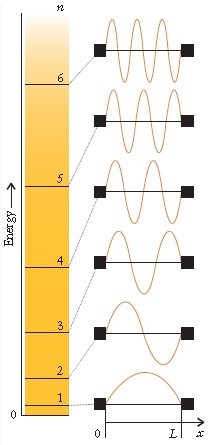
\includegraphics[width=0.25\textwidth]{images/figura1.png}
      \label{fig1}
    \end{figure}

    \par Pela definição clássica da funçaõ de onda $\Psi(\mathbf{x})$, temos:

    \begin{equation}\label{eq_schrodinger_eq2}
        \Psi (\mathbf{x}) = A \cdot sen(k \cdot \mathbf{x}) + B \cdot cos(k \cdot \mathbf{x})
    \end{equation}

    %TODO - QUAIS CONDIÇÕES SÃO ESSAS?
    \par Pela equação de Schrödinger, \eqref{eq_schrodinger_eq2} e das condições de contorno para o problema em questão, é possível concluir:

    \begin{equation}\label{eq_schrodinger_eq3}
      E = \frac{\hbar^2}{8 \pi^2 m} \cdot \frac{n^2\pi^2}{L^2} = \frac{\hbar^2 n^2}{8 m L^2},\ com\ n = 1, 2, ...
    \end{equation}

    \par Como $n \in \mathcal{Z} - \{0\}$, a equação \eqref{eq_schrodinger_eq3} mostra que somente alguns valores para energia são aceitos no confinamento dentro de uma caixa de tamanho L. A partir disso, conclui-se que os níveis de energia de uma partícula confinada são discretos e que a energia pode ser quantizada\cite{frustrado2}.

    \par Para definir o operador hamiltoniano utilizado para descrever partículas num cristal, começaremos do cristal perfeito, que descreve de maneira geral as relações entre as partículas nesse sistema. A partir dele, serão feitas aproximações para que se chegue no hamiltoniano do elétron livre\cite{qm_fis2}.

    \subsubsection{Hamiltoniano de um Cristal Perfeito}

      \par Para definir o operador hamiltoniano utilizado para descrever partículas num cristal, começaremos do cristal perfeito, que descreve de maneira geral as relações entre as partículas nesse sistema. A partir dele, serão feitas aproximações para que se chegue no hamiltoniano do elétron livre\cite{qm_fis2}. 
    
      \par O hamiltoniano do cristal perfeito\cite{frustrado3} é dado por:
      %TODO - REVISAR
      \begin{equation}\label{eq_schrodinger_eq4}
        \mathcal{H} = 
          \sum_{i} \frac{p_{i}^2}{2m_{i}} 
          + \sum_{j} \frac{p_{j}^2}{2m_{j}} 
          + \frac{1}{2} \sum_{j', j} \frac{Z_{j} Z_{j'} e^2}{4\pi\epsilon_{0}\left|R_{j} - R_{j'}\right|}-  \sum_{j, i} \frac{Z_{j} e^2}{4\pi\epsilon_{0}\left|r_{i} - R_{j}\right|} 
          + \frac{1}{2} \sum_{i, i'} \frac{e^2}{4\pi\epsilon_{0}\left|r_{i} - r_{i'}\right|}
      \end{equation}

      \par Na expressão \eqref{eq_schrodinger_eq4}, $\epsilon_{0}$ representa a permissividade no vácuo, $r_{i}$ representa a posição do i-ésimo elétron, $R_{j}$ representa a posição do j-ésimo núcleo, $Z_{j}$ representa o número atômico do núcleo, $p_{i}$ e $p_{j}$ representam o operador momento dos elétrons e o operador momento do núcleo, respectivamente. Além disso, os índices $i'$ e $j'$ são índices não identicos a $i$ e $j$.

      \par Para solucionar o hamiltoniano, leva-se em conta que os elétrons nas camadas totalmente preenchidas estão muito próximos ao núcleo, considerando-os como um pacote. Essa junção de elétrons mais internos com o núcleo atômico forma o que se chama por íon-núcleo.
    
      \par A partir disso, serão aplicadas duas aproximações para facilitar a solução do hamiltoniano. A primeira será a aproximação de Born-Oppenheimer.\cite{qm_fis9}


      \par Essa aproximação divide os átomos em duas grandes regiões. A primeira região trata o núcleo como uma partícula estática no espaço. Já a segunda região lida somente com as partículas na superfície do sistema.

      \par Aplicando a aproximação de Born-Oppenheimer ao hamiltoniano, pode-se separar os cálculos entre os íons-núcleo e os elétrons na camada de valência. Assim, simplifica-se o hamiltoniano como uma soma de hamiltonianos da relação entre os elétrons de valências, entre os íons-núcleo e entre ambas regiões, da seguinte maneira:

      \begin{equation}\label{eq_schrodinger_eq5}
        \mathcal{H} = 
          \mathcal{H}_{ions} (\mathbf{R}_{j}) 
          + \mathcal{H}_{e}(\mathbf{r}_{i}, \mathbf{R}_{j_{0}})
          + \mathcal{H}_{e-ion}(\mathbf{r}_i, \delta\mathbf{R}_j)
      \end{equation}

      \par Nessa expressão, $\mathcal{H}_{ions}(\mathbf{R}_{j})$ é o hamiltoniano referente às interações entre os íons-núcleo que se movimentam devido aos seus potenciais iônicos; $\mathcal{H}_{e}(\mathbf{r}_{i},\mathbf{R}_{j_{0}})$ é o hamiltoniano referente às interações elétron-elétron, considerando os íons-núcleo estáticos e congelados na posição de equilíbrio $\mathbf{R}_{j_{0}}$; $\mathcal{H}_{e-ion}(\mathbf{r}_{i},\delta\mathbf{R}_{j})$ é o hamiltoniano que descreve a interação elétron-íon, caracterizando a variação na energia eletrônica causada pelo deslocamento $\delta\mathbf{R}_{j}$ dos íons-núcleo em relação ao seu ponto de equilíbrio $\mathbf{R}_{j_{0}}$.
      
      \par Escrevendo o hamiltoniano do cristal perfeito, retirando os termos referentes unicamente ao núcleo e mantendo as interações elétron-elétron, obtém-se:

      \begin{equation}\label{eq_schrodinger_eq6}
        \mathcal{H}_{e} = 
          \sum_{i} \frac{p_{i}^2}{2m_{i}} 
          -  \sum_{j, i} \frac{Z_{j} e^2}{4\pi\epsilon_{0}\left|r_{i} - R_{j_{0}}\right|} 
          + \frac{1}{2} \sum_{i, i'} \frac{e^2}{4\pi\epsilon_{0}\left|r_{i} - r_{i'}\right|}
      \end{equation}

      \par Para simplificar a equação \eqref{eq_schrodinger_eq6}, será utilizada a aproximação \textit{mean-field}\cite{qm_fis10}. Essa aproximação consiste na escolha de um local arbitrário para o elétron no sistema e na consideração de que os outros graus de liberdade se encontram estáticos se utilizarmos seu valor médio. Aplicando o hamiltoniano somente em um elétron, tem-se que:

      \begin{equation}\label{eq_schrodinger_eq7}
        \mathcal{H}_{1e} = \frac{p^2}{2m}
      \end{equation}

      Considerando que o operador momento,na mecânica quântica, é definido por\cite{qm_fis11}:

      \begin{equation}\label{eq_schrodinger_eq8}
        p = -i\hbar\frac{d}{dx} \Longrightarrow
        p^2 = -\hbar^2 \frac{d^2}{dx^2} \Longrightarrow
        p^2 = -\hbar^2 \nabla^2
      \end{equation}

      Aplicando \eqref{eq_schrodinger_eq8} em \eqref{eq_schrodinger_eq7}, tem-se:

      \begin{equation}\label{eq_schrodinger_eq9}
        \mathcal{H}_{1e} = - \frac{\hbar^2}{2m}\nabla^2
      \end{equation}

      Define-se assim, o operador hamiltonia para o caso considerado. Aplicando a equação de Schrödinger ao caso do elétron livre, no qual o potencial U(\textbf{r}) é igual a zero, tem-se que:

      \begin{equation}\label{eq_schrodinger_eq10}
        \mathcal{H} \cdot \Psi(\mathbf{r}) =
          -\frac{\hbar^2}{2m} \nabla^2 \Psi(\mathbf{r}) =
          E \cdot \Psi(\mathbf{r})
      \end{equation}

      Com autovalores de energia dados por:

      \begin{equation}\label{eq_schrodinger_autovalores}
        E = \frac{\hbar^2 k^2}{2m}
      \end{equation}

      Em uma rede cristalina, o elétron sofre influência de um potencial. Esse potencial pode ser tratado como um potencial periódico\cite{qm_fis5} em alguns casos e será explicado a seguir.

  \subsection{Potencial Periódico e Teorema de Bloch}

    \par Para entender as propriedades eletrônicas dos pontos quânticos, uma análise de semicondutores Bulk (não confinados) é necessária. Como calcular o estado eletrônico para esses materiais é algo complexo, utilizam-se aproximações. Umas dessas aproximações consiste na observação do comportamento de um elétron, assumindo que todos os outros fazem parte dos íons que criam o potencial periódico.

\subsubsection{Potencial Periódico}

	\par A hamiltoniana\cite{qm_fis5} de um sólido contém tanto os potenciais monoeletrônicos quanto os potenciais de par. O primeiro descreve as interações dos elétrons com os núcleos e o segundo, as interações entre os elétrons. 

	\par Para o elétron independente, essas interações são representadas por um potencial efetivo monoeletrônico $U(\mathbf{r})$. Independente da forma desse potencial, se o cristal for perfeitamente periódico, ele deve satisfazer a seguinte equação:

	\begin{equation}
		\label{bloch_1}
		U(\mathbf{r}+\mathbf{R}) = U(\mathbf{R})
	\end{equation}

	Para o caso do elétron livre, $U(\mathbf{R})$ é zero, caracterizando o caso mais simples de um periódico. Assim, a equação de Schrödinger para o elétron livre se reduz à equação \eqref{bloch_1}. O vetor \textbf{r} está relacionado à célula primitiva, enquanto \textbf{R} indica os pontos de uma rede de Bravais\cite{qm_fis2}.

\subsubsection{Teorema de Bloch}

	\par O teorema de Bloch\cite{qm_fis5} afirma que os autoestados $\Psi$ podem ser escritos como uma onda plana vezes uma função de periodicidade para elétrons independentes, considerando que sobre eles atua um potencial periódico em uma rede de Bravais

	\begin{equation}
		\label{bloch_2}
		\Psi_{nk}(\mathbf{r})= e^{i\mathbf{k} \cdot \mathbf{r}}\cdot u_{nk}(\mathbf{r})
	\end{equation}

	As equações \eqref{bloch_1} e \eqref{bloch_2} implicam em:

	\begin{align}
		\label{bloch_3}
		\Psi_{nk}(\mathbf{R} + \mathbf{r}) &= e^{i\mathbf{k} \cdot \mathbf{r}}\cdot u_{nk}(\mathbf{R} + \mathbf{r})\\
		\Psi(\mathbf{R} + \mathbf{r}) &= e^{i\mathbf{k} \cdot \mathbf{R}}\cdot \Psi(\mathbf{r})
	\end{align}

	\par Os subíndices $n$ e $k$ serão explicados no final da prova do Teorema de Bloch, mas sua omissão não comprometará o entendimento do desenvolvimento a seguir.



	\subsubsection{Condição de Contorno de Born-Von Karman}

		\par Serão aplicadas as condições de contorno para que as funções de onda sejam periódicas.
		
		\par No caso tridimensional,

		\begin{align}\label{bloch_4}
	        \left\{
	          \begin{array}{ll}
	            \displaystyle \Psi(x+L, y, z) &= \Psi(x, y, z)\\
	            \displaystyle \Psi(x, y+L, z) &= \Psi(x, y, z)\\
	            \displaystyle \Psi(x, y, z+L) &= \Psi(x, y, z)
	          \end{array}
	        \right.
	      \end{align}
		
		\par A equação (2.5) é conhecida como condição de contorno de Born-Von Karman de periodicidade macroscópica.  Como nem sempre a rede de Bravais é cúbica, generaliza-se a condição de contorno para:

		\begin{equation}
			\label{blochh_5}
			\Psi(\mathbf{r} + N i\cdot \mathbf{a}_{i}) = \Psi(\mathbf{r}),\ i=1,2,3\ ,
		\end{equation}
		no qual $\mathbf{a}_{i}$ são os vetores primitivos da rede direta e $Ni$ são números inteiros, de forma que:

		\begin{equation}
			\label{bloch_6}
			N1 \cdot N2 \cdot N3 = N,
		\end{equation}
		onde N é o número total de células primitivas no cristal.

		\par Aplicando o Teorema de Bloch, obtém-se:

		\begin{equation}
			\label{bloch_7}
			\Psi(\mathbf{r} + Ni \cdot \mathbf{a}_{i}) = e^{i\cdot N i \cdot \mathbf{k} \cdot \mathbf{a}_{i}} \cdot \Psi(\mathbf{r})
		\end{equation}

		\par A equação \eqref{bloch_7} será válida para:

		\begin{equation}
			\label{bloch_8}
			e^{i\cdot N i \cdot \mathbf{k} \cdot \mathbf{a}_{i}} = 1,\ i=1,2,3
		\end{equation}

		\par A partir do mesmo desenvolvimento feito em \eqref{redeReciproca_eq6},

		\begin{equation}
			\label{bloch_9}
			\mathbf{k} \cdot \mathbf{a}_{i} = 2 \pi \mathbf{k} i
		\end{equation}

		\par Substituindo \eqref{bloch_9} em \eqref{bloch_8}, tem-se que:

		\begin{equation}
			\label{bloch_10}
			e^{i\cdot N i 2 \pi \cdot \mathbf{k} i} = 1
		\end{equation}

		\par Uma exponencial complexa pode ser escrita em função de senos e cossenos, através da fórmula de Euler. Observa-se que a relação acima será válida sempre que $2\pi$ estiver sendo multiplicado por um número inteiro. Como $Ni$ é um número inteiro e $\mathbf{k}i$ também, pode-se definir $\mathbf{k}i$ em função de $Ni$:

		\begin{equation}
			\label{bloch_11}
			\mathbf{k} = \sum_{i=1}^3 \frac{mi}{Ni} \cdot \mathbf{b}i,\ onde\ mi\ é\ inteiro.
		\end{equation}

		\par É definido que o elemento de volume, ou seja, o menor volume $\Delta\mathbf{k}$ da rede recíproca é formado pelo paralelepípedo com arestas $\frac{bi}{Ni}$, que pode ser escrito pelo produto misto:

		\begin{equation}
			\label{bloch_12}
			\Delta \mathbf{k} = \frac{\mathbf{b1}}{N1} \cdot \left( \frac{\mathbf{b2}}{N2} x \frac{\mathbf{b3}}{N3} \right)
				= \frac{1}{N} \cdot \mathbf{b1} \cdot \left(\mathbf{b2} x \mathbf{b3}\right)
		\end{equation}

		\par O vetor de onda pode ser escrito como $k=\frac{2\pi}{a}$, em que a é o parâmetro de rede da célula unitária. Assim, obtém-se $k^3=\frac{8\pi^3}{a^3}$, ou seja, $k^3=\frac{8\pi^3}{v}$, em que $v$ é o volume de uma célula primitiva na rede direta. Esse volume também é dado por $v=\frac{V}{N}$, onde $V$ representa o volume associado ao número de sítios da rede. Como o produto misto dos vetores $\mathbf{bi}$ representa o volume $k^3$. Logo, a equação \eqref{bloch_12} pode ser reescrita por:

		\begin{equation}
			\label{bloch_13}
			\Delta \mathbf{k} = \frac{8\pi^3}{V}
		\end{equation}

		\par Ao construir o teorema de Bloch para esse volume, ele se torna válido para toda a rede cristalina devido a sua periodicidade.

	\subsubsection{Prova do Teorema de Bloch}

	\par Para realizar a prova desse teorema, parte-se do princípio de que qualquer função que atenda às condições de Born-Von Karman pode ser expandida em ondas planas, sendo que essa expansão é feita por séries de Fourier. 
	
	\par Expandindo o potencial com periodicidade na rede de Bravais e a função de onda em ondas planas, obtém-se, respectivamente: 

	\begin{align}\label{bloch_14}
	      \begin{array}{ll}
	        \displaystyle U(\mathbf{r}) &= \sum_{\mathbf{K}} U_{\mathbf{K}} e^{i\mathbf{K}\cdot \mathbf{r}}\\
	        \displaystyle \Psi(\mathbf{r}) &= \sum_{\mathbf{K}} C_{\mathbf{k}} e^{i\mathbf{k}\cdot \mathbf{r}}	            
	      \end{array}
  \end{align}

	onde $C_{\textbf{k}}$ e $U_{\textbf{K}}$ são coeficientes.

	\par Assim, tem-se

	\begin{align}\label{bloch_15}
	      \begin{array}{ll}
	        \displaystyle \frac{\partial \Psi(\mathbf{r})}{\partial\mathbf{r}} &= \sum_{\mathbf{K}} C_{\mathbf{k}} ik e^{i\mathbf{k}\cdot \mathbf{r}}\\
	        \displaystyle \frac{\partial^2 \Psi(\mathbf{r})}{\partial\mathbf{r}^2} &= -\sum_{\mathbf{K}} C_{\mathbf{k}} k^2 e^{i\mathbf{k}\cdot \mathbf{r}}	            
	      \end{array}
  \end{align}

	Substituindo as equações de \eqref{bloch_15} na equação de Schrödinger \eqref{eq_schrodinger_frustrado}, tem-se que

	\begin{equation}
		\label{bloch_16}
		\sum_{\mathbf{K}} C_{\mathbf{k}} k^2 e^{i\mathbf{k}\cdot \mathbf{r}} \cdot \frac{\hbar}{2m}
			+ \sum_{\mathbf{K}} C_{\mathbf{k}} ik e^{i\mathbf{k}\cdot \mathbf{r}}
			= E \cdot \sum_{\mathbf{K}} C_{\mathbf{k}} e^{i\mathbf{k}\cdot \mathbf{r}}
	\end{equation}

	Reorganizando os termos para que se consiga colocar $e^{i\mathbf{k}\cdot \mathbf{r}}$ em evidência:

	\begin{equation}
		\label{bloch_17}
		\sum_{\mathbf{k}} e^{i\mathbf{k}\cdot \mathbf{r}}
			\left[ 
				C_\mathbf{k} \left( \frac{k^2 \hbar^2}{2m} - E \right)
				+ \sum_{\mathbf{K}} \mathbf{U}_{\mathbf{K}} \cdot C_{\mathbf{k-K}}
		   \right] = 0
	\end{equation}

	Como a equação \eqref{bloch_17} é válida para todo $\mathbf{r}$, então

	\begin{equation}
		\label{bloch_18}
		\left( \frac{k^2 \hbar^2}{2m} - E \right)
				+ \sum_{\mathbf{K}} \mathbf{U}_{\mathbf{K}} \cdot C_{\mathbf{k-K}} = 0
	\end{equation}

	\par A equação \eqref{bloch_18} é análoga à equação de Schrödinger só que para o espaço recíproco\cite{qm_fis2}. Um resultado importante obtido a partir dessa equação é que o coeficiente $C_{\mathbf{k}}$ se relaciona com os demais coeficientes\cite{qm_fis5}. Ou seja, $C\mathbf{k}$ acopla-se com $C_{\mathbf{k-K1}}$, $C_{\mathbf{k-K2}}$, etc. Isso significa que um ponto $C_{\mathbf{k}}$ da rede sofre influência de todos os outros pontos, gerando uma sobreposição das funções de onda. Isso fornece uma introdução aos níveis de energia\cite{bloch2}. É interessante observar que para $U_{\mathbf{K}} = 0$, a energia obtida é a do eĺétron livre.

	\par Pode reescrever a função de onda como:

	\begin{equation}
		\label{bloch_19}
		\Psi (\mathbf{r}) = \sum_{K} C_{\mathbf{k-K}}\cdot e^{i\mathbf{(k-K)}\cdot\mathbf{r}}
	\end{equation}

	\par Trazendo $e^{i\mathbf{k} \cdot \mathbf{r}}$ para fora do somatório:

	\begin{equation}
		\label{bloch_20}
		\Psi (\mathbf{r}) = e^{i\mathbf{k}\cdot\mathbf{r}} \cdot \left(\sum_{K} C_{\mathbf{k-K}}\cdot e^{-i \mathbf{K}\cdot\mathbf{r}}\right)
	\end{equation}

	\par Da equação \eqref{bloch_20}, tem-se que a função de periodicidade $u$ é dada por:

	\begin{equation}
		\label{bloch_21}
		u(\mathbf{r}) = \sum_{K} C_{\mathbf{k-K}}\cdot e^{-i \mathbf{K}\cdot\mathbf{r}}
	\end{equation}

	\par Assim, provou-se o teorema de Bloch, ao encontrar uma função de periodicidade $u$ que satisfaça a equação \eqref{bloch_1}.

	\par Como o problema foi analisado para um volume fixo, que diz respeito à região da célula unitária (equação \eqref{bloch_13}), tem-se infinitas soluções para k  com autovalores discretos, indexados pelo índice de bandas $n$. As energias $En(\mathbf{K})$ varia de forma contínua à medida que $\mathbf{k}$ varia e representam os níveis de energia para o elétron em um potencial periódico. Em relação a $n$, a energia varia de forma discreta. Ao atribuir os índices $n$ para as funções de onda e para os níveis de energia, obtém-se e $E n\mathbf{k}$. As informações que essas funções contêm são chamadas de estrutura de banda. Para cada $n$, o conjunto de níveis eletrônicos é chamado de banda de energia\cite{qm_fis5}. 



  \subsection{Teoria de Bandas nos Sólidos}

    \par A equação de Schrödinger mostra que átomos confinados possuem níveis de energia quantizados, conforme foi abordado anteriormente para o caso do elétron confinado em uma caixa. Num cristal, existem aproximadamente $10^{23}$ átomos por centímetro cúbico. Como os átomos em um material estão próximos um do outro, as funções de onda dos elétrons se superpõem, principalmente as dos elétrons da camada de valência. O princípio de exclusão de Pauli afirma que eles não podem ocupar os mesmos níveis de energia e, juntamente com a ação de um potencial, é criada uma distribuição de níveis, conhecida como banda de energia. As regiões energeticamente proibidas são chamadas de \textit{gaps} de energia\cite{qm_fis6}.

\subsection{Condutores, semicondutores e isolantes}

	\par As bandas de energia\cite{qm_fis6} são preenchidas de formas distintas para os diferentes tipos de materiais. O mapeamento das bandas de energia de ponto a ponto nas zonas de Brillouin gera estruturas de banda.

	\par Denomina-se por banda de condução, a banda de energia que é ocupada por elétrons que possuem energia maior que o nível de Fermi, promovendo a condutividade no material. Já a banda de valência é ocupada por elétrons que estão mais afastados do núcleo que os demais, sendo menos energética que a banda de condução.

	\begin{figure}[H]
      \caption{Bandas de energia para diferentes tipo de material (Adaptado de \cite{bulk1})}
      \centering
      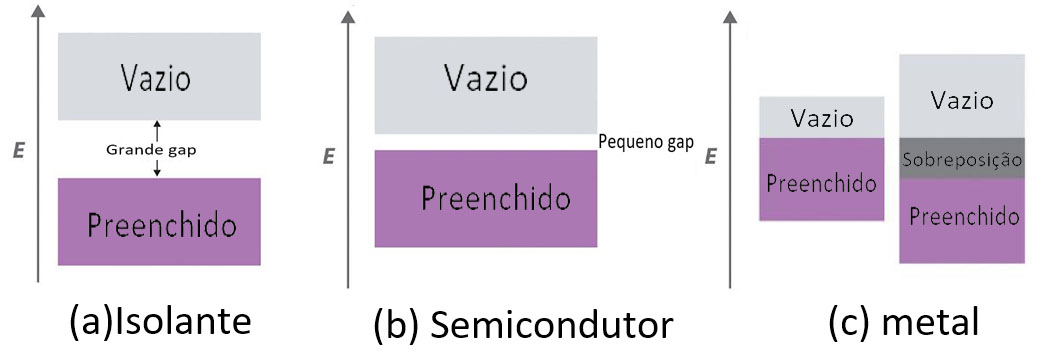
\includegraphics[width=0.75\textwidth]{images/figura3.jpg}
      \label{fig3}
    \end{figure}

	\par \textbf{Metais}
	
		\par Para que o elétron possa conduzir num metal ele precisa possuir energia acima da energia de fermi, Ef. Nesse tipo de material existem estados livres adjacentes aos estados com a energia de fermi, já que existe superposição entre as bandas de valência e condução. Portanto, muito pouca energia é necessária para que se faça um elétron de um metal conduzir. A figura \ref{fig3} ilustra as bandas de energia num metal. 

	\par \textbf{Isolantes}

		\par No caso dos isolantes existe um grande gap de energia entre as bandas de valência e condução, sendo necessária muita energia para que um elétron conduza. A figura \ref{fig4} ilustra as bandas de energia um isolante.

	\par \textbf{Semicondutores}
	
		\par Finalmente, para os semicondutores, categoria à qual os pontos quânticos pertencem, existe, como nos isolantes, um gap de energia entre as bandas de valência e condução. Porém, o gap para esses materiais é menor do que nos isolantes. Sendo assim, é possível que alguns elétrons da camada de valência saltem para a de condução se alguma energia for fornecida ao semicondutor. Essa energia pode ser, por exemplo, térmica ou eletromagnética. A figura \ref{fig5} ilustra as bandas de energia de um semicondutor.

\subsection{Semicondutores bulk}

	\par Quando as dimensões dos materiais são reduzidas à nanoescala, propriedades interessantes aparecem. O impacto desse confinamento depende de cada material e da propriedade a ser analisada. Para a análise das propriedades ópticas de nanocristais semicondutores, por exemplo, leva-se em consideração o raio de Bohr, pois essa dimensão descreve espacialmente os éxcitons. O confinamento espacial deles é conhecido como confinamento quântico e será abordado mais adiante. Para entendê-lo, é necessária uma abordagem da estrutura e das transições eletrônicas de semicondutores bulk. 

	\par \textbf{- Estrutura Eletrônica de Semicondutores bulk}

		\par Diferentemente do que ocorre para o elétron livre, um potencial periódico atua sobre o elétron em um semicondutor. Devido à periodicidade da rede e ao teorema de Bloch, sabe-se que a autofunção que satisfaz a propriedade de translação da rede é a função de onda de Bloch, definida anteriormente pela equação \eqref{bloch_3}.

		\par Novamente, para um elétron livre, a relação de dispersão é dada pela equação \eqref{eq_schrodinger_autovalores}, reescrita abaixo:

		\begin{equation}\label{eq_schrodinger_autovalores_rewrote}
	        E = \frac{\hbar^2 k^2}{2m}
	  	\end{equation}

	  	\par Essa relação pode ser observada na figura \ref{fig6}

	  	\begin{figure}[H]
	      \caption{(a) Dispersão de energia para um elétron livre. (b) Dispersão de energia para um elétron perturbado por um potencial periódico. (c) Banda de energia para a primeira zona de Brillouin.}
	      \centering
	      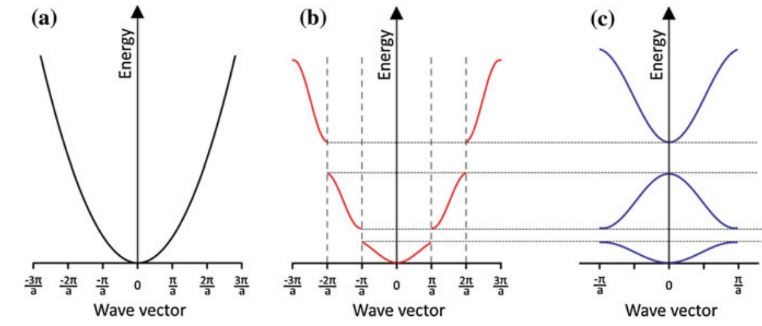
\includegraphics[width=0.75\textwidth]{images/figura6.jpg}
	      \label{fig6}
	    \end{figure}

	  	\par Ao perturbar a rede cristalina com um potencial periódico, ocorre uma mudança na relação de dispersão para o elétron. Essa perturbação provoca um gap de energia na região de degenerescência. Diz-se que um estado quântico é degenerado quando mais de uma função de onda está associada à mesma energia. Esse fenômeno pode ser observado na figura \ref{fig6}b. Os gaps de energia ocorrem para $\frac{n\pi}{a}$ porque os elétrons são refletidos, e essa reflexão é conhecida como reflexão de Bragg.

	  	\par A dispersão de energia pode ser restringida para valores de K entre $-\frac{n\pi}{a} < K < \frac{n\pi}{a}$, devido à periodicidade em K proporcionada pelo teorema de Bloch. Esse intervalo é conhecido como primeira zona de Brillouin. Quando a dispersão de energia é representada nela, tem-se a representação em zona reduzida. Considerando mais de um elétron nesse intervalo, configura-se a banda de energia, mostrada na figura \ref{fig6}c.

		\par Essa análise foi feita para o caso unidimensional. Para o caso tridimensional, a interpretação é mais complexa. Um exemplo desse último caso é mostrado na \ref{fig7}.

		\begin{figure}[H]
	      \caption{Estrutura de banda para o PbSe}
	      \centering
	      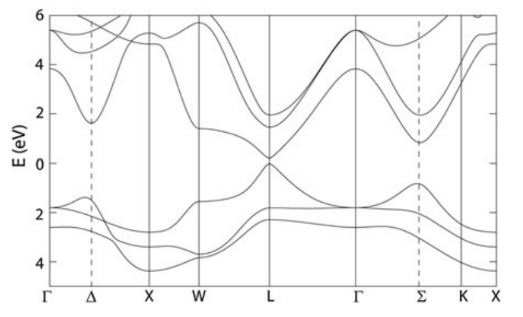
\includegraphics[width=0.75\textwidth]{images/figura7.jpg}
	      \label{fig7}
	    \end{figure}

		\par É válido ressaltar que  as estruturas de bandas também podem ser calculadas por modelos teóricos, como o método k.p e o DFT (teoria do funcional de densidade).

		\par O método utilizado para o cálculo da estrutura de banda dos pontos quânticos é o \textit{one-band mass efective model}\cite{bulk2}. Como o  grau de dificuldade desses métodos é alto, uma abordagem mais profunda sobre eles não será realizada neste trabalho.

	\par \textbf{- Transições eletrônicas para semicondutores bulk}

		\par Um semicondutor ideal na temperatura de zero Kelvin comporta-se como um isolante (estado fundamental). Ou seja, a banda de valência está totalmente preenchida e a banda de condução, vazia.
 		
 		\par Ao receber energia, alguns elétrons saltam para a banda de condução, fazendo com que buracos se desloquem para a banda de valência\cite{bloch1}. Buracos são orbitais vazios em uma banda de energia, que respondem a campos elétricos e magnéticos como se possuíssem carga +e\cite{qm_fis6}. O par elétron-buraco é chamado de éxciton e sua interação se dá pelo potencial de Coulomb\cite{bloch1}.

 		\par A energia mínima necessária para a formação do éxciton é dada por:

 		\begin{equation}
 			\label{bandas_1}
 			E = \hbar \omega = E_{g} + E_{e, kin} + E_{h, kin}
 		\end{equation}
 		onde $E_{g}$ representa o \textit{gap} de energia fundamental do semicondutor, $E_{e,kin}$ representa a energia cinética do elétron e $E_{h,kin}$, a energia cinética do buraco.

 		\par Da conservação de momento, tem-se:

 		\begin{equation}
 			\label{bandas_2}
 			\hbar \mathbf{k}_{cb} = \hbar \mathbf{k}_{vb} + \hbar \mathbf{k}_{foton}
 		\end{equation}

 		\par O termo $\mathbf{k}_{vb}$ é o vetor de onda para o elétron na banda de valência, $\mathbf{k}_{cb}$, o do buraco na banda de valência, e $\mathbf{k}_{foton}$, do fóton que tem momento despresível. Assim a relação $\mathbf{k}_{cb} = \mathbf{k}_{vb}$ deve ser satisfeita, como observado na figura \ref{fig8}

 		\begin{figure}[H]
	      \caption{Representação de um elétron absorvendo energia e saltando para a banda de condução. Forma-se um buraco na banda de valência.}
	      \centering
	      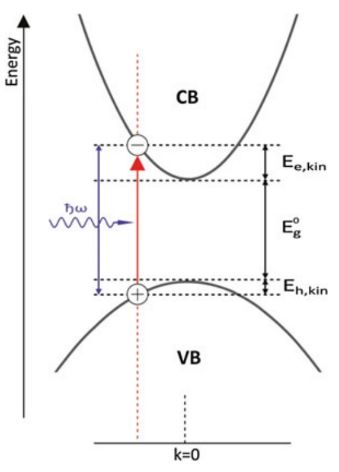
\includegraphics[width=0.35\textwidth]{images/figura8.jpg}
	      \label{fig8}
	    \end{figure}
